\chapter{Formulations faible et variationnelle}\label{Ch_FFaible}
\begin{abstract}
Un problème physique est généralement décrit par la donnée d'équations différentielles ou plus certainement aux dérivées partielles. Une telle formulation est appelée \textcolorblue{formulation forte} du problème.

Nous allons voir qu'il est possible d'exprimer ces équations différentielles ou équations aux dérivées partielles d'une manière «moins contraignante» pour les solutions recherchées. Une telle formulation sera qualifiée de formulation faible, et ses solutions appelées solutions faibles.

Évidemment, une solution forte du problème d'origine est également solution de la formulation faible.
\end{abstract}


\medskip
\section{Principe des formulations faible et variationnelle}\index{formulation faible}
Quand on cherche la solution d'une équation aux dérivées partielles, on peut être confronté aux problèmes suivants:
\begin{itemize}
  \item La solution ou les coefficients de l'équation aux dérivées partielles linéaires peuvent ne pas être assez réguliers pour donner un sens classique à l'équation;
  \item La solution peut être régulière mais l'espace de régularité en question n'a pas les bonnes propriétés pour obtenir directement l'existence de la solution dans cet espace.
\end{itemize}


\medskip
On va donc essayer de donner un sens plus faible à la notion de solution, sans perdre de vue si possible les notions les plus naturelles. Donner un sens faible à une équation aux dérivées partielles signifie:
\begin{enumerate}
  \item Chercher une solution dans un espace de régularité plus faible que souhaité;
  \item Établir, en général à l'aide de fonction tests et d'intégrations par parties «formelles», une série d'équations que doit vérifier cette solution. Cette série  d'équations doit être construite (si possible) de telle sorte que les éventuelles 	solutions régulières soient aussi solutions faibles et, a contrario, que des solutions faibles qui seraient régulières soient aussi solutions classiques du problème initial.
\end{enumerate}


\medskip
Les difficultés d'une telle approche sont nombreuses:
\begin{itemize}
  \item Le choix de l'espace fonctionnel dans lequel on va chercher la solution est crucial, pas toujours unique et parfois non trivial.
  \item Si l'on affaiblit trop la notion de solution, il sera \emph{a priori} plus facile de démontrer l'existence mais les propriétés d'unicité seront plus difficiles à obtenir.
  \item Si l'on n'affaiblit pas suffisamment l'équation, l'existence sera ardue à prouver mais l'unicité sera plus simple.
\end{itemize}


\medskip
Il s'agit donc de trouver un juste équilibre...

Dans le cas des équations elliptiques, celles-ci ont pour propriété, en général, de mettre en jeu des dérivées d'ordre pair de la solution dans le terme principal de l'équation. L'idée première pour résoudre ces problèmes aussi bien d'un point de vue théorique que numérique va être de multiplier formellement l'équation par une fonction test régulière, puis d'intégrer sur le domaine et enfin d'intégrer par parties un nombre suffisant de fois pour faire porter autant de dérivées sur la solution que sur les fonctions tests. On pourra ainsi envisager d'utiliser le même espace fonctionnel pour la solution et les fonctions tests.

\bigskip
Étant donné un opérateur différentiel~$A(\cdot)$ et une fonction~$f$ définie sur un domaine ouvert~$\Omega$, la \textcolorblue{formulation forte} du problème est la suivante:
\begin{center}
  Trouver la \textcolorblue{fonction}~$u$ définie sur~$\Omega$ vérifiant~$A(u)=f$ en tout point de~$\Omega$.
\end{center}

\medskip
Une solution~$u$ du problème précédent est alors également solution du problème suivant
appelé \textcolorblue{formulation faible} (On appelle~$v$ une fonction test):
\begin{center}
  Trouver une fonction~$u$ définie sur~$\Omega$ vérifiant~$\dint_\Omega A(u),\quad v = \int_\Omega f\ v$
$\forall v$ définie sur~$\Omega$.
\end{center}


\colorgreen%
\paragraph{Justification}
Tout réside dans le fait de «multiplier par une fonction test et d'intégrer».
Pourquoi peut-on faire ça ?
%Pourquoi les solutions aux deux problèmes sont-elles les mêmes ?

Partons de l'équation forte:
\begin{equation}A(u)=f,\quad \forall x\in\Omega\end{equation}
Nous pouvons multiplier les deux membres de l'équation par une fonction~$v$ à condition que cette fonction~$v$ ne soit pas identiquement nulle. Dans ce cas, la solution de 
\begin{equation}A(u)v=f\cdot v,\quad \forall x\in\Omega\end{equation} 
est la même~$\forall v$ suffisamment sympathique.
Comme cette seconde équation est vraie en tout point de~$\Omega$, alors elle est encore vraie sous forme intégrale, i.e. sous forme faible, à condition que $v$ soit suffisamment régulière pour pouvoir être intégrée.

On entrevoit alors clairement la suite des opérations: si en plus d'être régulière, la fonction~$v$ est différentiable, alors on va pouvoir réaliser sur le terme~$\int A(u)\cdot v$ une intégration par parties pour diminuer les conditions de dérivabilité portant sur~$u$, mais en augmentant celles portant sur~$v$.

Si l'ordre de dérivation de~$u$ est paire (disons~$2k$), alors on pourra faire en sorte par un nombre suffisant de manipulations que~$u$ et~$v$ aient à être différentiables à l'ordre~$k$... et on pourra essayer de faire en sorte que~$u$ et~$v$ appartiennent au même espace fonctionnel...

\medskip
\colorgris
Petit aparté sur d'autres manières de présenter «la chose»: en mécanique, on parle également du «principe du travail virtuel» (ou des puissances virtuelles), de «minimisation de l'énergie potentielle», ou encore de «méthode des résidus pondérés»,
Toutes ces méthodes sont «équivalentes» à celle exposée ici, mais souvent leur démonstration se fait uniquement «par les mains», ce qui peut être frustrant.

\medskip
\paragraph{Principe des puissances virtuelles}\index{principe!des puissances virtuelles}\index{principe!des travaux virtuels}
Le Principe des travaux virtuels est un principe fondamental en mécanique, qui postule un équilibre de puissance dans un mouvement virtuel, il s'agit d'une formulation duale du principe fondamental de la dynamique. On raisonne comme suit: si un solide est à l'équilibre (statique du solide), la somme des efforts est nulle. Donc si l'on fait faire un déplacement fictif (virtuel) à l'objet, la somme des puissances des forces et moments est nulle. Ce principe constitue la base d'une démarche de modélisation pour les milieux continus (théorie du premier gradient, théorie du second gradient). On parle parfois du principe des travaux virtuels qui est sensiblement identique.



\medskip



\begin{histoire}%
L'origine de ce principe revient à Jean Bernoulli\index[aut]{Bernoulli (Jean), 1667-1748, Suisse},\index[aut]{Bernoulli (Jean), 1667-1748, Suisse} qui énonce en 1725 le principe des vitesses virtuelles, qui consiste à considérer la perturbation de l'équilibre d'un système mécanique par un mouvement infinitésimal respectant les conditions de liaison du système, un mouvement virtuel, et d'en déduire une égalité de puissance.

\sbox{\MaBoiteAvecPhotos}{\setlength{\tabcolsep}{0pt}\scriptsize%
\begin{tabular}{ccc}%c}
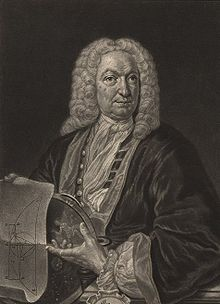
\includegraphics[height=\the\HauteurDesPhotos]{Bernoulli-Jean}&
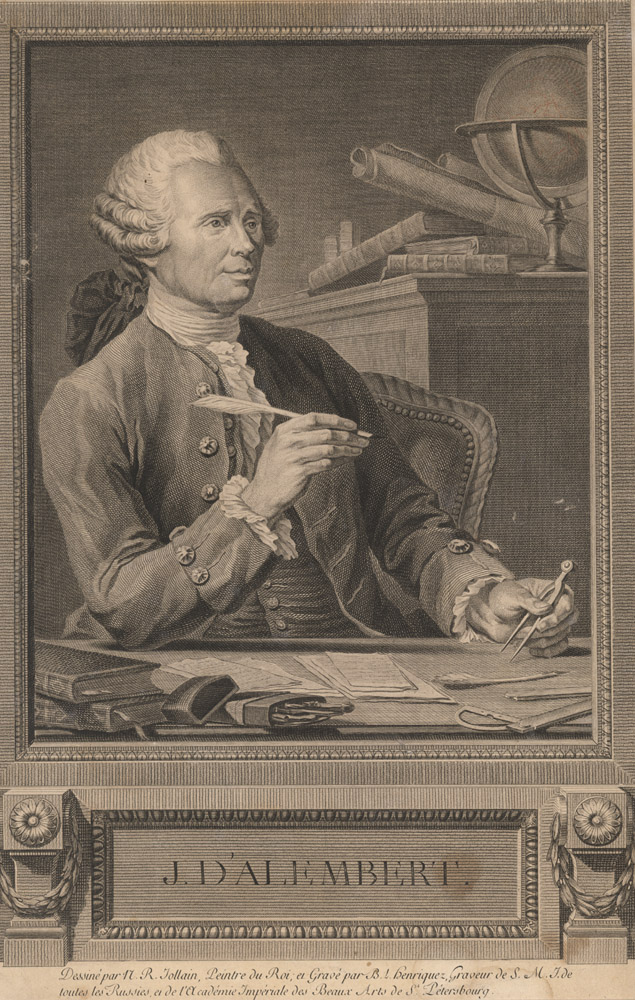
\includegraphics[height=\the\HauteurDesPhotos]{dAlembert2}&
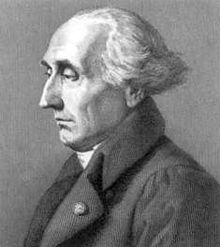
\includegraphics[height=\the\HauteurDesPhotos]{Lagrange3}\\
%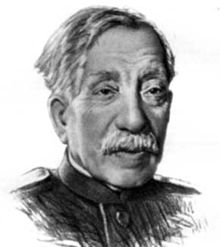
\includegraphics[height=\the\HauteurDesPhotos]{Galerkine}\\
J. Bernoulli &D'Alembert&Lagrange% & Galerkine%
\end{tabular}}
\medskip
\ImageADroite{%
Ce principe a été par la suite généralisé par D'Alembert\index[aut]{d'Alembert (Jean le Rond), 1717-1783, Français} et Lagrange\index[aut]{Lagrange (Joseph Louis, comte de -), 1736-1813, Italien} en ce qui est connu actuellement sous le nom de principe de D'Alembert (1743).\index{principe! de d'Alembert}

Le principe des puissances virtuelles est une synthèse de ces principes, ancrée dans un cadre beaucoup plus rigoureux et mathématique (on parle alors de «dualisation» et non plus de «perturbation» de l'équilibre ou du mouvement par un mouvement infinitésimal).}
\end{histoire}

\colorgris
\medskip
\paragraph{Minimisation de l'énergie potentielle}\index{énergie potentielle}
L'énergie potentielle d'un système physique est l'énergie liée à une interaction, qui a le «potentiel» de se transformer en énergie cinétique.

Cette énergie est une fonction de ce système, dépendant des coordonnées d'espace, et éventuellement du temps, ayant la dimension d'une énergie et qui est associée à une force dite conservative dont l'expression s'en déduit par dérivation (ce qui veut dire au passage que dans les cas où toutes les forces ne sont pas conservatives, par exemple s'il y a du frottement, alors la méthode ne fonctionne pas et doit être «adaptée»). La différence entre les énergies potentielles associées à deux points de l'espace est égale à l'opposé du travail de la force concernée pour aller d'un point à l'autre, et ce quel que soit le chemin utilisé.

\medskip
\paragraph{Méthode des résidus pondérés}\index{résidus pondérés}\label{Sec-ResPond}
Si l'on considère l'équation~$A(u)=f, \forall x\in\Omega$ sur~$\Omega$, on appelle résidu des équations d'équilibre la quantité~$R(x)=A(u)-f$. Aux bords, on a les conditions $B(u)=h, \forall x\in\Gamma=\partial\Omega$, et on appelle résidu des équations de bords la quantité~$\overline{R}(x)=B(u)-h$. En écrivant le problème dans~$\Omega$ et sur son contour~$\Gamma$ de manière intégrale, on retombe sur une formulation faible.

La méthode des résidus pondérés consiste à calculer les composantes de la solution approchée par la projection sur des couples de fonctions de projection, appelées fonctions de pondération.

Selon les fonctions de pondération on retrouve les méthodes de collocation par sous-domaine (fonctions constante sur chaque sous-domaine), de collocation par point (fonctions non nulles en un seul point), des fonctions splines (en ajoutant des conditions des raccordements des fonctions et des dérivées), de Galerkine\index[aut]{Galerkine (Boris), 1871-1945, Russe} (mêmes fonctions pour les fonctions de forme et de pondération).
\colorblack

\medskip
Selon la nature du problème (donc selon la nature de l'opérateur~$A$), l'égalité précédente (la formulation faible) peut être transformée (par exemple par intégration par parties), ce qui permet de faire apparaître une forme symétrique ayant la nature d'un produit scalaire (ou d'un produit hermitien\index[aut]{Hermite (Charles), 1822-1901, Français} dans le cas de fonctions complexes). Les deux fonctions~$u$ et~$v$ appartiennent alors à un même espace fonctionnel.

\medskip
La \textcolorblue{formulation variationnelle} d'un problème régi par des équations aux dérivées partielles correspond à une formulation faible de ces équations qui s'exprime en termes d'algèbre linéaire dans le cadre d'un espace de Hilbert.

Il n'y a donc fondamentalement \textcolorred{pas de différence entre formulation faible et formulation variationnelle}, sauf que cette dernière appellation est généralement réservée à des cas «qui vont bien»... et de manière très pragmatique aux cas où la formulation faible peut être transformée en un problème de minimisation: on dit alors qu'il existe une \textcolorblue{fonctionnelle}~$\Pi$ dont la \textcolorgreen{variation}~$\delta\Pi$ correspond au problème faible, d'où le terme de formulation variationnelle \textcolorgreen{(d'un point de vue physique, la fonctionnelle représente l'énergie du système, et le lieu où sa variation est nulle $\delta\Pi=0$ l'état recherché)}.

\medskip
Par ailleurs, d'autres contraintes sur la frontière de~$\Omega$ peuvent (doivent) être imposées à~$u$ (et à~$v$). Ce sont les \textcolorblue{conditions aux limites}.
%Nous allons présenter ces conditions aux limites maintenant.
Les conditions aux limites types ont été présentées au chapitre précédent.

\medskip
\section{Théorème de représentation de Riesz-Fréchet}\index{théorème!de représentation de Riesz-Fréchet}\index[aut]{Riesz (Frigyes), 1880-1956, Hongrois}\index[aut]{Fréchet (Maurice René), 1878-1973, Français}
Le théorème le plus fondamental sera le théorème de Lax-Milgram, toutefois, nous aurons besoin du théorème de représentation de Riesz-Fréchet pour sa démonstration.

\medskip
Pour tout vecteur~$y$ d'un espace de Hilbert~$H$, la forme linéaire qui à~$x$ associe~$\langle y,x\rangle$ est continue sur~$H$ (sa norme est égale à celle de~$y$, d'après l'inégalité de Cauchy-Schwarz). Le théorème de Riesz énonce la réciproque: toute forme linéaire continue sur~$H$ s'obtient de cette façon.

\medskip
\subsection{Cas des formes linéaires}

\begin{theoreme}[Théorème de représentation de Riesz-Fréchet]\label{Th-RF}
%\colorblue
Soient~$H$ un espace de Hilbert (réel ou complexe) muni de son produit scalaire noté $\langle\cdot,\cdot\rangle$ et~$f \in H'$ une forme linéaire continue sur~$H$.
Alors il existe un unique~$y$ dans~$H$ tel que pour tout~$x$ de~$H$ on ait~$f(x)=\langle y,x\rangle$.
\begin{equation}
\exists\,!\ y \in H\,, \quad \forall x\in H\,, \quad f(x) = \langle y,x\rangle
\end{equation}
\end{theoreme}
\colorblack

\medskip
\subsection{Extension aux formes bilinéaires}

\colorgris%
Si~$a$ est une forme bilinéaire continue sur un espace de Hilbert réel~$H$ (ou une forme sesquilinéaire complexe continue sur un Hilbert complexe), alors il existe une unique application $A$ de~$H$ dans~$H$ telle que, pour tout~$(u,v)\in H\times H$ on ait $a(u,v)=\langle Au,v \rangle$.

De plus, $A$ est linéaire et continue, de norme égale à celle de~$a$.
\begin{equation}
\exists !\,A\in \mathcal{L}(H),\quad \forall (u,v)\in H\times H,\quad a(u,v)=\langle Au,v \rangle
\end{equation}
\colorblack

\medskip
\section{Théorème de Lax-Milgram}\index{théorème!de Lax-Milgram}\label{Sec-ThLaxMilgram}\index[aut]{Lax (Peter), 1926-, Américain}\index[aut]{Milgram (Arthur Norton), 1912-1961, Américain}\label{Sec:LaxMil}

\medskip
\begin{definition}[Continuité d'une forme linéaire]
Une forme bilinéaire~$a$ est dite \textcolorblue{continue} si elle vérifie:
\begin{equation}
\exists\,c>0,\quad \forall (u,v)\in H^2\,,\quad |a(u,v)|\leq c\|u\|\|v\|
\end{equation}
\end{definition}

\medskip
\begin{definition}[Coercitivité d'une forme linéaire]
Une forme bilinéaire~$a$ est dite \textcolorblue{coercitive} si elle vérifie:
\begin{equation}
\exists\,\alpha>0,\quad \forall u\in H\,,\quad a(u,u) \geq \alpha\|u\|^2
\end{equation}
\end{definition}

\begin{theoreme}[Théorème de Lax-Milgram]
Soit~$H$ un espace de Hilbert réel ou complexe muni de son produit scalaire noté $\langle\cdot,\cdot\rangle$, de norme associée~$\|\cdot\|$.

Soit~$a(\cdot,\cdot)$ une forme bilinéaire (ou une forme sesquilinéaire dans le cas complexe) continue et coercitive sur~$H\times H$, et soit~$f$ une forme linéaire continue sur~$H$ (i.e. $f\in H'$).

Alors il existe un unique~$u$ dans~$H$ tel que l'équation~$a(u,v) = f(v)$ soit vérifiée~$\forall v \in H$.
\begin{equation}
  \exists!\ u \in H,\quad \forall v\in H,\quad a(u,v)=f(v)
\end{equation}
\colorblack
\end{theoreme}


\medskip
{\noindent\footnotesize\colorgris
\textbf{Preuve}\hskip5pt
La continuité et la coercitivité de~$a$ permettent de dire que~$a$ définit un produit scalaire~$(\cdot,\cdot)_a$ dont la norme associée~$\|\cdot\|_a$ est équivalente à la norme~$\|\cdot\|$. 
Le problème devient: trouver~$u$ tel que~$\forall v\in H, (u,v)_a=f(v)$.

Or~$f(v)=<f,v>$ dans la dualité~$H$~$H'$ et le problème devient:
trouver~$u$ tel que~$\forall v\in H, (u,v)_a=<f,v>$.

Le théorème de représentation de Riesz-Fréchet permet de conclure à l'existence et à l'unicité de la solution.~$\square$

\noindent
Une autre preuve consiste à étudier directement le problème de minimisation de la fonctionnelle \textcolorblue{$J=\frac12 a(v,v)-f(v)$} (ce qui est une façon de montrer le théorème de Riesz) en considérant une suite minimisante et en montrant qu'elle est de Cauchy par l'identité du parallélogramme.~$\square$
\colorblack}


\medskip
\textcolorred{Ce théorème est l'un des fondements de la méthode des éléments finis} dits «classiques» ou «en déplacement». Dans le cas d'éléments finis plus «exotiques» tels que les éléments mixtes, hybrides, mixtes-hybrides et des multiplicateurs de Lagrange, on a besoin d'un peu plus... c'est ce que nous allons voir au paragraphe suivant.


\begin{theoreme}[Forme variationnelle du théorème du Lax-Milgram]
Si de plus la forme bilinéaire~$a$ est symétrique, alors~$u$ est l'unique élément de~$H$ qui minimise la fonctionnelle
$J: H\rightarrow\RR$ définie par~$J(v) = \frac12 a(v,v)-f(v)$ pour tout~$v$ de~$E$:
\begin{equation}
\exists!\ u \in H,\quad J(u) = \min_{v\in H}\ J(v) = \min_{v\in H} \left( \frac12 a(v,v) - f(v) \right)
\end{equation}
\end{theoreme}


\medskip
\colorgreen
Pour les problèmes issus de la mécanique des solides déformables, la quantité~$\frac12 a(v,v)$ représente l'énergie de déformation du solide associé à un «déplacement virtuel»~$v$, et~$f(v)$ l'énergie potentielle des forces extérieures appliquées au solide pour le même déplacement virtuel~$v$.
\colorblack


\medskip
\section{Théorème de Babuška et condition inf-sup}\index{théorème!de Babuška}\label{Sec-ThBabuska}\index[aut]{Babuška (Ivo Milan), 1926-, Tchèque}
\textcolorgreen{Il s'agit d'une situation introduite en 1971/72 par Babuška.}

\textcolorgreen{Le but est d'étendre le théorème de Lax-Milgram aux problèmes non nécessairement coercitifs (i.e. la forme bilinéaire n'est plus supposée coercitive).}

\medskip
\begin{theoreme}[Théorème de Babuška]
Soient~$H$ et~$M$ deux espaces de Hilbert.
Soient~$a(\cdot,\cdot)$ une forme bilinéaire continue sur~$H \times M$ et~$f(\cdot)$ une forme linéaire continue sur~$M$.
On s'intéresse au problème: Existe-t-il~$u\in H$ tel que~$a(u,v)=f(v)$, $\forall v\in M$ ?

Si~$a(\cdot,\cdot)$ vérifie:
\begin{equation}\left\{
\begin{aligned}
&\displaystyle\inf_{\substack{u\in H\\\|u\|_H=1}} \sup_{\substack{v\in M\\\|v\|_M=1}} a(u,v) > 0\\[+2mm]
&\displaystyle\sup_{\substack{u\in H\\\|u\|_H=1}} a(u,v) > 0, \quad\forall v\in M\backslash\{0\}\\
\end{aligned}\right.
\end{equation}
Alors~$\forall f\in M'$, le problème admet une unique solution~$u$.
\end{theoreme}
\colorblack

\medskip
La première condition s'écrit aussi:
\begin{equation}
\exists \beta > 0, \sup_{\substack{v\in M\\\|v\|_M=1}} a(u,v) \ge \beta \|u\|_H, \forall u\in H
\end{equation}
Alors que le seconde s'écrit:
\begin{equation}
\forall v\in M\backslash\{0\},\quad \exists u\in H,\quad a(u,v)>0
\end{equation}


\medskip
\textcolorgris{La preuve du théorème de Babuška revient à montrer que l'opérateur~$A$ associé à la forme bilinéaire~$a$ est un homéomorphisme.}


\section{Théorèmes de Brezzi et condition BBL}\index{théorème!de Brezzi}\index{condition BBL}\label{Sec-ThBrezzi}

\index[aut]{Brezzi (Franco), 1945-, Italien}\label{Sec:Brezzi}
\textcolorgreen{Il s'agit d'étendre le théorème de Lax-Milgram au cas où, cette fois, le problème n'est plus écrit à l'aide d'une seule variable ($u$ jusqu'à présent), mais à l'aide de plusieurs variables. Dans ce cas, on parle de \textcolorblue{formulation mixte.}}

\medskip
\begin{theoreme}[Théorème de Brezzi (1974)]
%\colorblue
Considérons le problème variationnel mixte suivant:
Trouver ($u, \lambda)$ dans~$H\times M$ tels que:
 \begin{equation}\label{Eq-PM}\left\{
\begin{array}{rcl}
 a(u,v) + b(v, \lambda) &=& \langle f,v\rangle \quad \forall v\in H,\\
b(u,\mu) &=& \langle g,\mu\rangle \quad \forall \mu \in M.
\end{array}\right.
\end{equation}

Si les conditions suivantes sont satisfaites:
\begin{itemize}
%  \item~$f\in X'$, $g\in M'$;
  \item~$a(\cdot,\cdot)$ est continue;
  \item~$a(\cdot,\cdot)$ est coercitive sur~$V$ ou~$V$-elliptique (uniquement sur~$V$ et pas sur~$H$ tout entier) \textcolorgris{(sur~$\ker B$)}:
  \begin{equation}\exists \alpha> 0 \text{ tel que: } a(v,v)\ge\alpha\|c\|^2, \quad \forall v\in V=\{v\in H; b(v,\mu)=0, \forall \mu\in M \}\end{equation}
  \item~$b(\cdot,\cdot)$ est continue;
  \item~$b(\cdot,\cdot)$ vérifie la condition inf-sup suivante:
\begin{equation}\inf_{\substack{\mu\in M\\\|\mu\|_M=1}} \sup_{\substack{v\in H\\\|v\|_H=1}} b(v,\mu) > 0\end{equation}
\end{itemize}
Alors, $\forall (f,g)\in H'\times M'$, le problème précédent possède une unique solution
$(u,\lambda) \in H\times M$.
\end{theoreme}
\colorblack

\medskip
\textcolorgreen{%
On dit condition inf-sup ou condition de Brezzi, ou condition de Babuška-Brezzi-Ladyjenskaïa, ou condition BBL.}\index{condition inf-sup}\index[aut]{Ladyjenskaïa (Olga Aleksandrovna), 1922-2007, Russe}\index[aut]{Brezzi (Franco), 1945-, Italien}\index[aut]{Babuška (Ivo Milan), 1926-, Tchèque}


La condition de~$V$-ellipticité s'écrit également:
\begin{equation}\inf_{v\in V\backslash\{0\}} a(v,v)>0 \end{equation}
et la condition BBL:
\begin{equation}
\exists \beta > 0,\quad \sup_{v\in H} \dfrac{b(v,\mu)}{\|v\|_H}\ge \beta \|\mu\|_M,\quad \forall \mu\in M
\end{equation}


\medskip
On va écrire la démarche de la démonstration car elle est typique de la résolution de ce genre de problème.

\colorgris{\footnotesize\noindent\textbf{Preuve:}
On va se servir de~$H=V\oplus V^\bot$ avec~$V=\ker B$ où évidemment~$B$ est l'opérateur définit de~$H$ dans~$M'$ tel que:~$\langle Bu,\mu\rangle_M=b(u,\mu)$, $\forall\mu\in M$. Pour le produit scalaire induit, $V$ et~$V^\bot$ sont des Hilbert.

La solution cherchée est~$u=u_0+u_\bot$.

Les inconnues seront donc~$u_0$, $u_\bot$ et~$\lambda$.

On a les équations pour~$v_0$, $v_\bot$ et~$\mu$.
Pour~$v_\bot$ l'équation est:
\begin{equation}\left\{
\begin{array}{rcll}
a(u_\bot,v_\bot)+a(u_0,v_\bot)+b(v_\bot,\lambda) &=& \langle f,v_\bot\rangle &\forall v_\bot\in V^\bot\\
a(u_\bot,v_0)+a(u_0,v_0)+b(v_0,\lambda) &=& \langle f,v_0\rangle &\forall v_0\in V\\
b(u_\bot,\mu)+b(u_0,\mu) &=& \langle g,\mu\rangle &\forall \mu\in M
\end{array}
\right.\end{equation}
Or dans la seconde équation, $b(v_0,\lambda)=0$ car~$v_0\in\ker b$ et dans l'équation 3, $b(u_0,\mu)=0$
car~$u_0\in V$.

On est ramené à 3 sous-problèmes:
\begin{itemize}
  \item sous-problème 1: chercher~$u_\bot\in V^\bot$ tel que~$b(u_\bot,\mu)=g(\mu)$, $\forall\mu\in M$,
	ce qui est effectivement le cas d'après le théorème de Babuška;
  \item sous-problème 2: chercher~$u_0\in V$ tel que~$a(u_0,v_0)=\langle f,v_0\rangle-a(u_\bot,v_0)$,
	$\forall v_0\in V$.
	Il suffit de vérifier que le second membre définit un opérateur tel que l'on a bien les
	hypothèses du théorème de Lax-Milgram;
  \item sous-problème 3: chercher~$\lambda\in M$ tel que~$b(v_\bot,\lambda)=\langle f,v_\bot\rangle-a(u,v_\bot)$,
	$\forall v_\bot\in V^\bot$.
	Il faut un peu plus travailler pour vérifier que l'on est dans le cas d'application du théorème de Babuška, mais ça se
	fait (une quinzaine de lignes en détail).
\end{itemize}
}\colorblack



\medskip
On peut remplacer les conditions de~$V$-ellipticité sur~$a(\cdot,\cdot)$ par des conditions de Babuška.

\medskip
\begin{theoreme}[Théorème généralisé de Brezzi]
\index{théorème!de Brezzi!généralisé}\index[aut]{Brezzi (Franco), 1945-, Italien}
Considérons le problème variationnel mixte suivant:
Trouver ($u, \lambda)$ dans~$H\times M$ tels que:
 \begin{equation}\left\{
\begin{array}{rcl}
 a(u,v) + b(v, \lambda) &=& \langle f,v\rangle \quad \forall v\in H,\\
b(u,\mu) &=& \langle g,\mu\rangle \quad \forall \mu \in M.
\end{array}\right.
\end{equation}
Si les conditions suivantes sont satisfaites:
\begin{itemize}
  \item~$a(\cdot,\cdot)$ est continue;
  \item~$a(\cdot,\cdot)$ vérifie les deux conditions suivantes:
  \begin{equation}\exists \alpha> 0 \text{ tel que: } \sup_{v\in V\backslash\{0\}} \frac{a(u,v)}{\|v\|} \ge\alpha\|u\|_H^2, \quad \forall u\in V=\ker B\end{equation}
 ~$\forall v\in V\backslash\{0\}, \exists u\in V, a(u,v)\ne 0~$ ou de manière équivalente
~$\displaystyle\forall v\in V\backslash\{0\}, \sup_u a(u,v)> 0~$
  \item~$b(\cdot,\cdot)$ est continue;
  \item~$b(\cdot,\cdot)$ vérifie la condition inf-sup suivante:
\begin{equation}\inf_{\substack{\mu\in M\\\|\mu\|_M=1}} \sup_{\substack{v\in H\\\|v\|_H=1}} b(v,\mu) > 0\end{equation}
\end{itemize}
Alors, $\forall (f,g)\in H'\times M'$, le problème précédent possède une unique solution
$(u,\lambda) \in H\times M$.
\end{theoreme}
\colorblack
Pour vérifier la condition LBB, il est souvent plus simple de vérifier le critère suivant:
La condition inf-sup sur~$b(\cdot,\cdot)$ est équivalente à:
\begin{equation}\colorred
\forall\mu\in M, \exists v\in H \text{ (uniquement dans } V^\bot\text{) tel que: }
b(v,\mu)=\|\mu\|^2 \text{ et } \|v\|\le \dfrac1\beta \|\mu\|
\end{equation}









\medskip
\section{Multiplicateurs de Lagrange}\index{multiplicateurs de Lagrange}\index[aut]{Lagrange (Joseph Louis, comte de -), 1736-1813, Italien}\label{Sec-MultLag}
Nous avons déjà présenté les multiplicateurs de Lagrange d'un point de vue pratique au chapitre précédent. Regardons maintenant l'aspect mathématique.

Dans les paragraphes~\ref{Sec-ThLaxMilgram} et~\ref{Sec-ThBabuska} sur les théorèmes de Lax-Milgram et de Babuška, nous avons traité le cas d'un problème décrit par un seul champ inconnu. Dans le paragraphe~\ref{Sec-ThBrezzi} sur le théorème de Brezzi, nous avons traité le cas d'un problème formulé avec deux champs inconnus (mais on pourrait l'étendre à autant de champs que nécessaire).
Dans ce paragraphe, nous allons traiter un cas un peu «au milieu»: par exemple deux domaines possédant chacun leur formulation, mais couplés. Il est donc nécessaire dans ce cas d'introduire une «équation de couplage» entre ces formulations. C'est ce que l'on se propose de réaliser à l'aide des multiplicateurs de Lagrange.

\medskip
\begin{definition}[Formulation comme problème de minimisation sous contrainte]
Soient~$H$ et~$M$ deux espaces de Hilbert.
Soient~$a(\cdot,\cdot): H\times H\rightarrow\RR$ une forme bilinéaire \textcolorred{symétrique et continue}
et~$b(\cdot,\cdot): H\times M\rightarrow\RR$ une forme bilinéaire \textcolorred{continue}.
Soient enfin~$f\in H'$ et~$g\in M'$ deux formes linéaires. On notera
$\langle\cdot,\cdot\rangle_H$ et~$\langle\cdot,\cdot\rangle_M$ les produits de dualité entre~$H$ et~$H'$
et entre~$M$ et~$M'$ respectivement.

\medskip
On considère le problème suivant:
\begin{equation}
\begin{array}{c}
\text{Trouver } u\in H \text{ tel que } a(u,v)=f(v), \forall v\in H \\
\text{ \textcolorred{et} vérifiant les
\textcolorblue{contraintes} supplémentaires: } b(v,\mu)=g(\mu), \forall \mu\in M.
\end{array}
\end{equation}

\medskip
Ce problème est équivalent à:
\begin{equation}\label{Eq-Pmin}
\begin{array}{c}
\text{Trouver} u\in H \text{ tel que }
J(u)=\min\{J(v), v\in H \text{ et } b(v,\mu)=\langle g,\mu\rangle_M, \mu\in M\} \\[+3mm]
\text{ avec }
J(v)=\frac12 a(v,v)-\langle f,v\rangle_H
\end{array}
\end{equation}
%On notera ce problème (Pmin), et
On parle de \textcolorblue{problème de minimisation sous contrainte}.
\end{definition}

\medskip



On introduit un \textcolorblue{Lagrangien}:
$\mathscr{L}(v,\mu) = J(v)+b(v,\mu) - \langle g,\mu\rangle_M$.
Évidemment, $\forall\mu, \mathscr{L}(v,\mu)=J(v)$ si~$v$ vérifie les contraintes.
L'idée est de considérer~$\min_{v\in H} \mathscr{L}(v,.)$.
La question devient alors: \textcolorblue{existe-t-il un multiplicateur particulier~$\lambda\in M$ tel que
~$\min_{v\in H} \mathscr{L}(v,\lambda)$ soit égale à~$u\in H$ solution de (\ref{Eq-Pmin})?}
\textcolorgreen{$\lambda$ est parfois également appelé pénalité ou fonction de pénalisation.}


\medskip



En notant que:
\begin{equation}\langle\frac{\partial\mathscr{L}}{\partial v}(u,\lambda),v\rangle_H
=\frac d{dt}\mathscr{L}(y+tv,\lambda)|_{t=0}
=a(u,v)-\langle f,v\rangle_H+b(v,\lambda)
\end{equation}
Alors~$(u,\lambda) \in H\times M$ est solution du problème mixte (\ref{Eq-PM}):
 \begin{equation}\left\{
\begin{array}{rcl}
 a(u,v) + b(v, \lambda) &=& \langle f,v\rangle \quad \forall v\in H,\\
b(u,\mu) &=& \langle g,\mu\rangle \quad \forall \mu \in M.
\end{array}\right.
\end{equation}
et \textcolorred{on se retrouve dans le cadre du théorème de Brezzi} au paragraphe~\ref{Sec-ThBrezzi}.

\medskip
De plus, si~$a(v,v)\ge 0$, $\forall v\in H$, alors~$(u,\lambda)$ est solution de (\ref{Eq-PM}) correspond à~$(u,\lambda)$ est un \textcolorblue{point-selle} de~$\mathscr{L}$, i.e.:
\begin{equation}
\forall\mu\in M, \mathscr{L}(u,\mu) \le \mathscr{L}(u,\lambda) \le
\mathscr{L}(v,\lambda), \forall v\in H
\end{equation}


\medskip
Remarquons enfin que si l'on note:
\begin{align}&A((u,\lambda),(v,\mu))=a(u,v)+b(v,\lambda)+b(u,\mu)\\
&L((v,\mu))=f(v)+g(\mu)\end{align}
et que l'on pose les nouvelles variables~$\mathscr{U}=(u,\lambda)$ et~$\mathscr{V}=(v,\mu)$, alors \textcolorred{on revient à un problème de type Lax-Milgram}: trouver~$\mathscr{U}\in H\times M$
tel que pour tout~$\mathscr{V}\in H\times M$, $A(\mathscr{V},\mathscr{U})=L(\mathscr{V})$.
%\newpage% Pour version livre du 20130712

\begin{histoire}%
Comme nous l'avons déjà mentionné, Lagrange\index[aut]{Lagrange (Joseph Louis, comte de -), 1736-1813, Italien} est le fondateur du calcul des variations avec Euler.\index[aut]{Euler (Leonhard Paul), 1707-1783, Suisse}

\sbox{\MaBoiteAvecPhotos}{\setlength{\tabcolsep}{0pt}\scriptsize%
\begin{tabular}{c}%
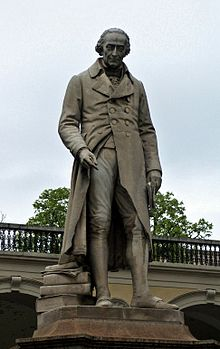
\includegraphics[height=32mm]{Lagrange4}\\%
Lagrange%
\end{tabular}}
\medskip
\ImageADroite{%
Il est également le fondateur de la théorie des formes quadratiques, et démontre le théorème de Wilson\index[aut]{Wilson (John), 1741-1793, Anglais} sur les nombres premiers et la conjecture de Bachet\index[aut]{Bachet (Claude-Gaspard, dit - de Mérizac), 1581-1638, Français} sur la décomposition d'un entier en quatre carrés (connu aussi sous le nom de théorème des quatre carrés de Lagrange). On lui doit un cas particulier du théorème auquel on donnera son nom en théorie des groupes, un autre sur les fractions continues, l'équation différentielle de Lagrange.\index[aut]{Lagrange (Joseph Louis, comte de -), 1736-1813, Italien}\\
\indent
En physique, en précisant le principe de moindre action, avec le calcul des variations, vers 1756, il invente la fonction de Lagrange,\index[aut]{Lagrange (Joseph Louis, comte de -), 1736-1813, Italien} qui vérifie les équations de Lagrange, puis développe la mécanique analytique, vers 1788, pour laquelle il introduit les multiplicateurs de Lagrange.\index{multiplicateurs de Lagrange} Il entreprend aussi des recherches importantes sur le problème des trois corps en astronomie, un de ses résultats étant la mise en évidence des points de libration (dits points de Lagrange) en 1772.\\
\indent
En mécanique des fluides, il introduisit le concept de potentiel de vitesse en 1781, bien en avance sur son temps. Il démontra que le potentiel de vitesse existe pour tout écoulement de fluide réel, pour lequel la résultante des forces dérive d'un potentiel. Dans le même mémoire de 1781, il introduisit, en plus, deux notions fondamentales: le concept de la fonction de courant, pour un fluide incompressible, et le calcul de la célérité d'une petite onde dans un canal peu profond. Rétrospectivement, cet ouvrage marqua une étape décisive dans le développement de la mécanique des fluides moderne.}
\end{histoire}
